\documentclass[a4paper,10pt]{article}
%\documentclass[dutch]{IEEEtran}
%\documentclass[a4paper,10pt]{scrartcl}
\usepackage{pdfpages} 
%\usepackage[dutch]{babel}
\usepackage[english]{babel}
\usepackage[utf8]{inputenc}
\usepackage[official]{eurosym}
\usepackage{listings}
\usepackage[titles]{tocloft}
\usepackage{amssymb,amsmath}
%\usepackage{caption}
\usepackage{url}
\usepackage[nottoc, numbib]{tocbibind}
\usepackage{gensymb}
\usepackage{placeins}
\usepackage{float}
%\usepackage[style=ieee, backend=bibtex]{biblatex}
 
\title{Quantified Bike}
\author{Lies Bollens \and Jakob Festraets \and Rugen Heidbuchel \and Floris Kint \and Peter Lacko}
\date{\today}

\pdfinfo{%
  /Title    (Quantified Bike)
  /Author   (Team CWA3: Lies Bollens, Ruben De Clercq, Jakob Festraets, Rugen Heidbuchel, Floris Kint, Peter Lacko)
  /Creator  ()
  /Producer ()
  /Subject  ()
  /Keywords ()
}
\setlength{\footskip}{100pt}
\begin{document}
%\maketitle
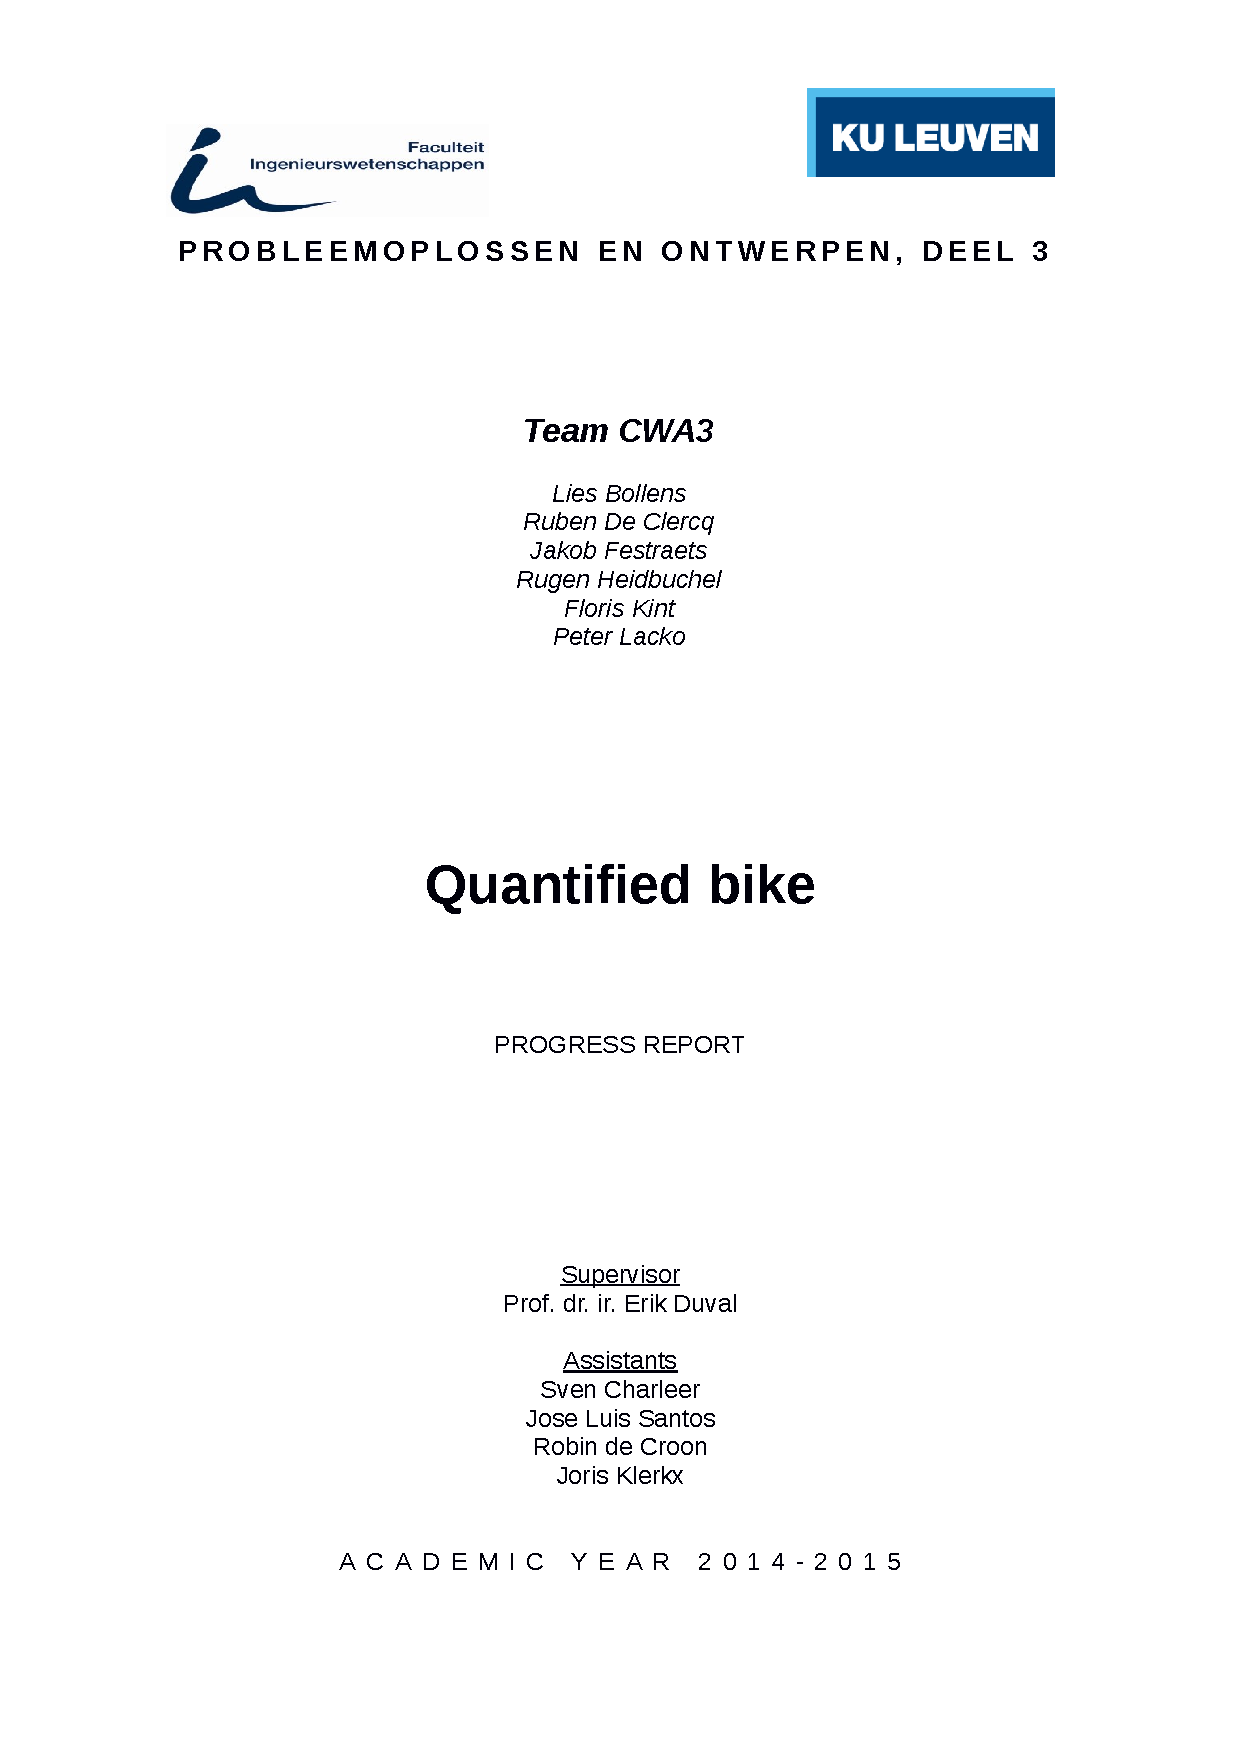
\includepdf[pages={-},pagecommand={}]{voorbladtv1415.pdf}
\newpage
\tableofcontents
\newpage
\listoffigures
%\newpage
%\listoftables
\newpage
%\section{Conclusion}
We already learned a lot in this project. First of all, we learned how to combine an
Arduino with a Raspberry Pi. Secondly, we learned a lot about web technologies. We now
know how to write webpages using the combination of HTML, CSS and javascript (with
jQuery). Thirdly, we learned how to use the version management system called git.

We think the introduction sessions where good. They weren't too long and gave a short summary of what every technology was meant for.Those who didn't know these
technologies yet, could go through some tutorials. The only thing we did not like about the project, was the focus on 
a quantified bike. We would have prefered a combination of a quantified and an augmented bike, since an augmented bike
has a lot more applications in real-life. It would be easier to imagine a user public and to implement a useful application.

We still plan to make use of SCSS, to easily change global parameters like our base colour.

\section{Conclusion}
We already learned a lot in this project. First of all, we learned how to combine an
Arduino with a Raspberry Pi. Secondly, we learned a lot about web technologies. We now
know how to write webpages using the combination of HTML, CSS and javascript (with
jQuery). Thirdly, we learned how to use the version management system called git.

We think the introduction sessions where good. They weren't too long and gave a short summary of what every technology was meant for.Those who didn't know these
technologies yet, could go through some tutorials. The only thing we did not like about the project, was the focus on 
a quantified bike. We would have prefered a combination of a quantified and an augmented bike, since an augmented bike
has a lot more applications in real-life. It would be easier to imagine a user public and to implement a useful application.

We still plan to make use of SCSS, to easily change global parameters like our base colour.

\section{Conclusion}
We already learned a lot in this project. First of all, we learned how to combine an
Arduino with a Raspberry Pi. Secondly, we learned a lot about web technologies. We now
know how to write webpages using the combination of HTML, CSS and javascript (with
jQuery). Thirdly, we learned how to use the version management system called git.

We think the introduction sessions where good. They weren't too long and gave a short summary of what every technology was meant for.Those who didn't know these
technologies yet, could go through some tutorials. The only thing we did not like about the project, was the focus on 
a quantified bike. We would have prefered a combination of a quantified and an augmented bike, since an augmented bike
has a lot more applications in real-life. It would be easier to imagine a user public and to implement a useful application.

We still plan to make use of SCSS, to easily change global parameters like our base colour.

\section{Conclusion}
We already learned a lot in this project. First of all, we learned how to combine an
Arduino with a Raspberry Pi. Secondly, we learned a lot about web technologies. We now
know how to write webpages using the combination of HTML, CSS and javascript (with
jQuery). Thirdly, we learned how to use the version management system called git.

We think the introduction sessions where good. They weren't too long and gave a short summary of what every technology was meant for.Those who didn't know these
technologies yet, could go through some tutorials. The only thing we did not like about the project, was the focus on 
a quantified bike. We would have prefered a combination of a quantified and an augmented bike, since an augmented bike
has a lot more applications in real-life. It would be easier to imagine a user public and to implement a useful application.

We still plan to make use of SCSS, to easily change global parameters like our base colour.

\section{Conclusion}
We already learned a lot in this project. First of all, we learned how to combine an
Arduino with a Raspberry Pi. Secondly, we learned a lot about web technologies. We now
know how to write webpages using the combination of HTML, CSS and javascript (with
jQuery). Thirdly, we learned how to use the version management system called git.

We think the introduction sessions where good. They weren't too long and gave a short summary of what every technology was meant for.Those who didn't know these
technologies yet, could go through some tutorials. The only thing we did not like about the project, was the focus on 
a quantified bike. We would have prefered a combination of a quantified and an augmented bike, since an augmented bike
has a lot more applications in real-life. It would be easier to imagine a user public and to implement a useful application.

We still plan to make use of SCSS, to easily change global parameters like our base colour.

\section{Conclusion}
We already learned a lot in this project. First of all, we learned how to combine an
Arduino with a Raspberry Pi. Secondly, we learned a lot about web technologies. We now
know how to write webpages using the combination of HTML, CSS and javascript (with
jQuery). Thirdly, we learned how to use the version management system called git.

We think the introduction sessions where good. They weren't too long and gave a short summary of what every technology was meant for.Those who didn't know these
technologies yet, could go through some tutorials. The only thing we did not like about the project, was the focus on 
a quantified bike. We would have prefered a combination of a quantified and an augmented bike, since an augmented bike
has a lot more applications in real-life. It would be easier to imagine a user public and to implement a useful application.

We still plan to make use of SCSS, to easily change global parameters like our base colour.

\section{Conclusion}
We already learned a lot in this project. First of all, we learned how to combine an
Arduino with a Raspberry Pi. Secondly, we learned a lot about web technologies. We now
know how to write webpages using the combination of HTML, CSS and javascript (with
jQuery). Thirdly, we learned how to use the version management system called git.

We think the introduction sessions where good. They weren't too long and gave a short summary of what every technology was meant for.Those who didn't know these
technologies yet, could go through some tutorials. The only thing we did not like about the project, was the focus on 
a quantified bike. We would have prefered a combination of a quantified and an augmented bike, since an augmented bike
has a lot more applications in real-life. It would be easier to imagine a user public and to implement a useful application.

We still plan to make use of SCSS, to easily change global parameters like our base colour.

\section{Conclusion}
We already learned a lot in this project. First of all, we learned how to combine an
Arduino with a Raspberry Pi. Secondly, we learned a lot about web technologies. We now
know how to write webpages using the combination of HTML, CSS and javascript (with
jQuery). Thirdly, we learned how to use the version management system called git.

We think the introduction sessions where good. They weren't too long and gave a short summary of what every technology was meant for.Those who didn't know these
technologies yet, could go through some tutorials. The only thing we did not like about the project, was the focus on 
a quantified bike. We would have prefered a combination of a quantified and an augmented bike, since an augmented bike
has a lot more applications in real-life. It would be easier to imagine a user public and to implement a useful application.

We still plan to make use of SCSS, to easily change global parameters like our base colour.

\section{Conclusion}
We already learned a lot in this project. First of all, we learned how to combine an
Arduino with a Raspberry Pi. Secondly, we learned a lot about web technologies. We now
know how to write webpages using the combination of HTML, CSS and javascript (with
jQuery). Thirdly, we learned how to use the version management system called git.

We think the introduction sessions where good. They weren't too long and gave a short summary of what every technology was meant for.Those who didn't know these
technologies yet, could go through some tutorials. The only thing we did not like about the project, was the focus on 
a quantified bike. We would have prefered a combination of a quantified and an augmented bike, since an augmented bike
has a lot more applications in real-life. It would be easier to imagine a user public and to implement a useful application.

We still plan to make use of SCSS, to easily change global parameters like our base colour.

\section{Conclusion}
We already learned a lot in this project. First of all, we learned how to combine an
Arduino with a Raspberry Pi. Secondly, we learned a lot about web technologies. We now
know how to write webpages using the combination of HTML, CSS and javascript (with
jQuery). Thirdly, we learned how to use the version management system called git.

We think the introduction sessions where good. They weren't too long and gave a short summary of what every technology was meant for.Those who didn't know these
technologies yet, could go through some tutorials. The only thing we did not like about the project, was the focus on 
a quantified bike. We would have prefered a combination of a quantified and an augmented bike, since an augmented bike
has a lot more applications in real-life. It would be easier to imagine a user public and to implement a useful application.

We still plan to make use of SCSS, to easily change global parameters like our base colour.

\section{Conclusion}
We already learned a lot in this project. First of all, we learned how to combine an
Arduino with a Raspberry Pi. Secondly, we learned a lot about web technologies. We now
know how to write webpages using the combination of HTML, CSS and javascript (with
jQuery). Thirdly, we learned how to use the version management system called git.

We think the introduction sessions where good. They weren't too long and gave a short summary of what every technology was meant for.Those who didn't know these
technologies yet, could go through some tutorials. The only thing we did not like about the project, was the focus on 
a quantified bike. We would have prefered a combination of a quantified and an augmented bike, since an augmented bike
has a lot more applications in real-life. It would be easier to imagine a user public and to implement a useful application.

We still plan to make use of SCSS, to easily change global parameters like our base colour.


\bibliographystyle{IEEEtran}
\bibliography{referenties}{}

\end{document}
